\documentclass[a4paper,12pt]{article}

\usepackage{amsmath,amssymb,amsfonts,euscript,mathrsfs,wasysym,textcomp,pifont}
\usepackage{psfrag}
\usepackage[dvips]{graphicx}
\usepackage[usenames]{color}
\usepackage{fullpage}

\pagestyle{empty}

\begin{document}

\psfrag{pL}[tc][tc][1.]{$x^{\rm L}$}
\psfrag{pU}[tc][tc][1.]{$x^{\rm U}$}
\psfrag{p}[Bc][Bc][1.]{$x$}
\psfrag{pref1}[Bc][Bc][1.]{$\color{red}\hat{x}_1$}
\psfrag{pref2}[Bc][Bc][1.]{$\color{red}\hat{x}_2$}
\psfrag{pref3}[Bc][Bc][1.]{$\color{red}\hat{x}_3$}
\psfrag{f}[Bl][Bl][1.]{$\color{red}f$}
\psfrag{pf}[tc][tc][1.]{$\mathcal P$}
\psfrag{pf(p)+R}[tc][tc][1.]{$\color{blue}\mathcal P(\hat x_2)\oplus\mathcal R$}
\psfrag{pf+rU}[bl][bl][1.]{$\color{blue}\mathcal P+r^{\rm U}$}
\psfrag{pf+rL}[bl][bl][1.]{$\color{blue}\mathcal P+r^{\rm L}$}
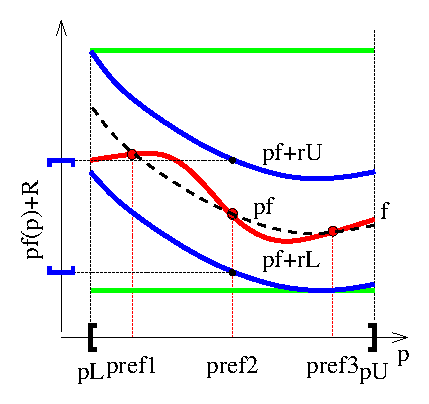
\includegraphics[width=.45\textwidth]{Chebyshevmodel.eps}

\end{document}
